% !TEX root = ./rosbook_jp.tex
%-------------------------------------------------------------------------------
\chapterimage{chapter_head_6.pdf}

%-------------------------------------------------------------------------------
\chapter{ROSプログラミングの基本}

%-------------------------------------------------------------------------------
\section{メッセージ、トピック、サービス、パラメータ}\index{メッセージ、トピック、サービス、パラメータ}

5章まではROSの概要や、コマンド、ツールなどを紹介した。本章からは本格的にROSプログラミングについて説明していく。
ここまでで最も頻繁に使われた用語は、メッセージ、トピック、サービス、パラメータなどである。ROSプログラミングにおける最小の実行単位であるノードは、メッセージ通信を介してほかのノードとデータをやり取りするが、それに使用される方式がトピック、サービスである。一方、パラメータ通信は、パラメータサーバとノード間でパラメータ値をやり取りする際に用いられる。本節では、メッセージ通信、パラメータ通信の概念、および具体的な通信方式を、実例を交えて説明する。

\begin{definition*}[ROSで使用される通信]
ROSで使用される通信には、ノード間でメッセージをやり取りするメッセージ通信と、パラメータサーバとノード間でパラメータ値をやり取りするパラメータ通信    がある。図6-1にメッセージ通信とパラメータ通信の概要を示す 。メッセージ通信は、一方向通信方式のトピック(topic)通信と、双方向通信方式のサービス(service)通信に分けることができる。
\end{definition*}

\begin{figure}[h]
  \centering
  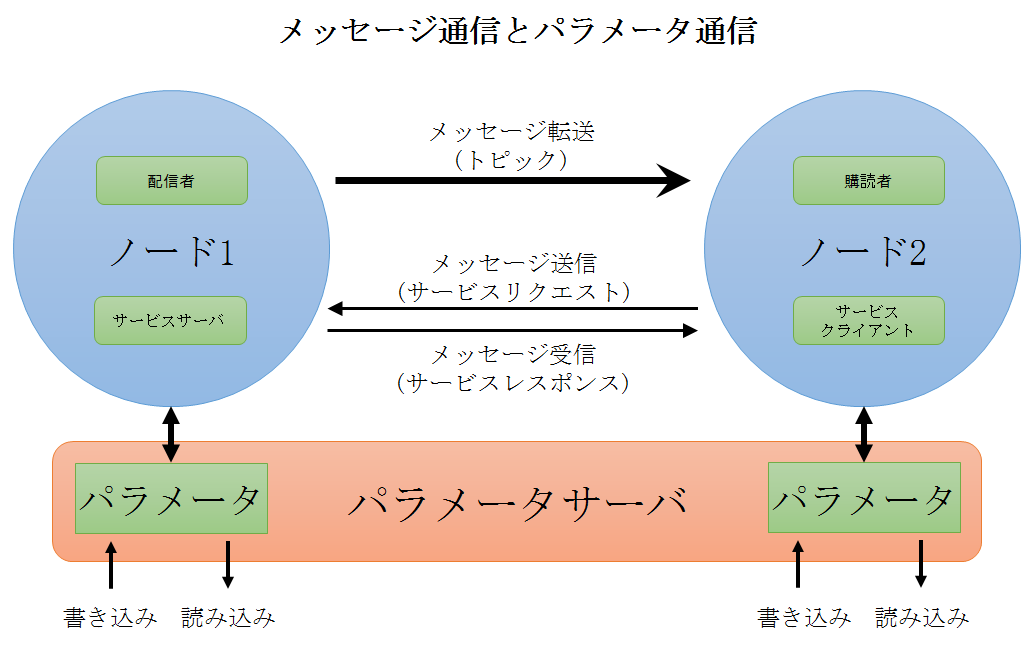
\includegraphics[width=10cm]{pictures/chapter6/pic_06_01.png}
  \caption{ノード間のメッセージ通信とパラメータ通信}
\end{figure}

\begin{definition*}[トピック(topic)通信]
トピック通信とは、ノードからノードへ一方向にメッセージを送信する手段である。この時、メッセージを配信するノードを配信者(publisher)ノード、購読するノードを購読者(subscriber)ノードという。配信者ノードはメッセージを配信する際に、マスターにトピック名を登録する。トピック(話題)とはメッセージの内容を表すラベルである。トピックの購読を購読者ノードが希望すると、マスターはそのトピックを配信している配信者ノードの情報を購読者ノードに伝える。この情報をもとに、購読者ノードと配信者ノードは直接通信を行う。
トピック通信は一方向通信であるが、一回接続された配信者ノードと購読者ノードは、その後は連続して通信を行うことができるという特徴をもつ。そのため、センサからセンサドライバを通して直接計測値を読み込むノードを配信者ノード、計測値を加工してより高度な情報処理を行うノードを購読者ノードとするなど、連続してメッセージを送る必要があるセンサデータ送信に適している。
\end{definition*}

\begin{figure}[h]
  \centering
  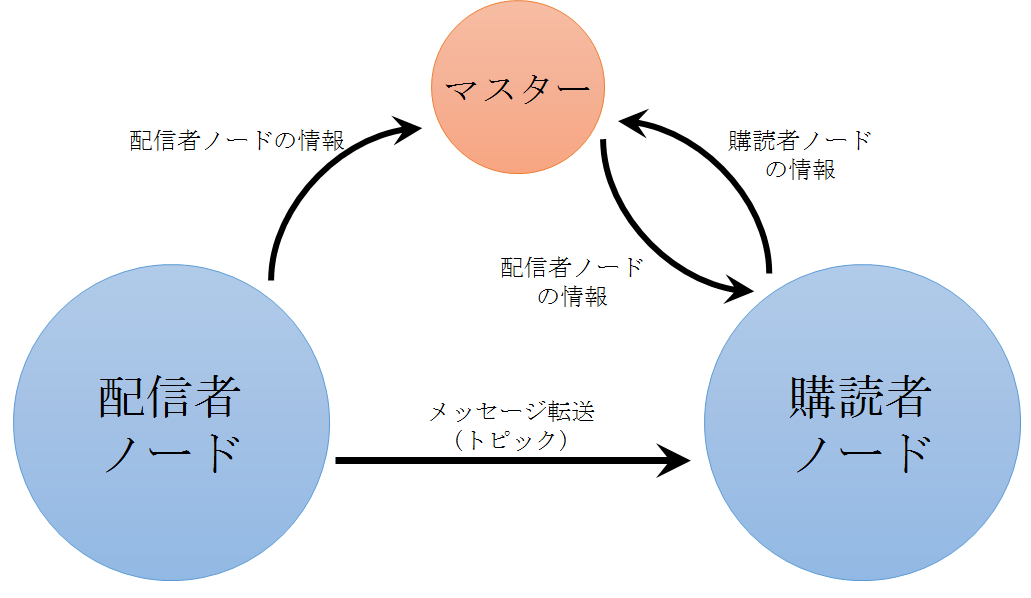
\includegraphics[width=10cm]{pictures/chapter6/pic_06_02.png}
  \caption{トピック通信}
\end{figure}

\begin{definition*}[サービス(service)通信]
サービス通信   とは、ノード間でリクエスト/レスポンス方式でメッセージをやり取りする手段である。リクエストを送り、レスポンスを待つノードをサービスクライアント(service client)、リクエストを受けた後、レスポンスを返すノードをサービスサーバ(service server)という。サービスサーバは起動と同時に、マスターにサービス名を登録する。サービスクライアントがサービスリクエストを送る際、マスターはそのサービスサーバの情報をサービスクライアントに伝える。その後、サービスクライアントはサービスサーバと直接接続し、サービス通信を行う。
サ  ービスは、トピックとは異なり、一回限りのメッセージ通信であるため、サービスのリクエストとレスポンスが完了すると、2つのノードの接続は切断される。  サービス通信は、ロボットへの定型動作の実行命令や、特定の条件が満たされたときにイベントを発生するノードなどに使用される。
\end{definition*}

\begin{figure}[h]
  \centering
  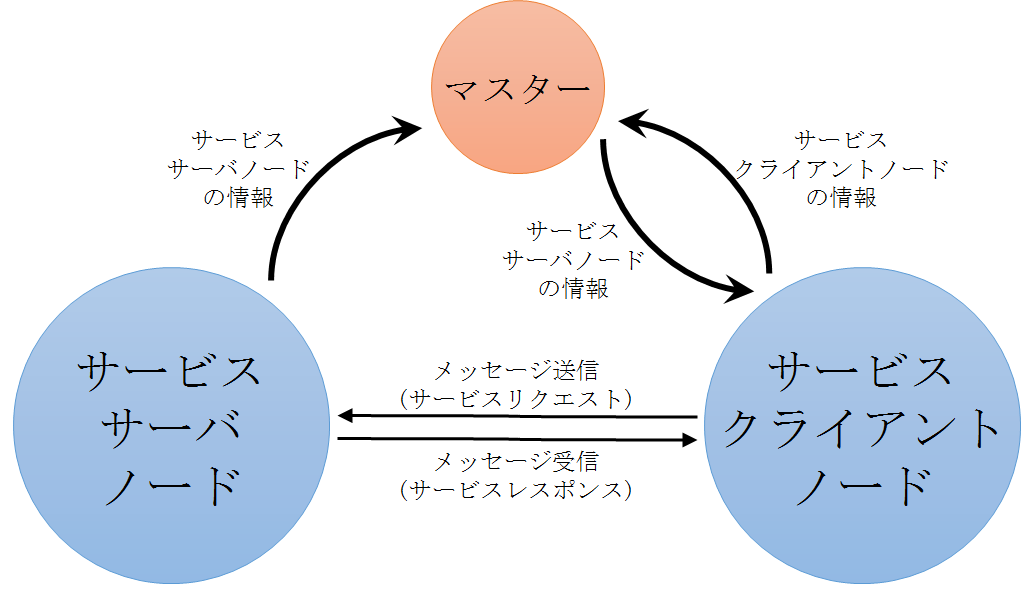
\includegraphics[width=10cm]{pictures/chapter6/pic_06_03.png}
  \caption{サービス通信}
\end{figure}

\begin{definition*}[パラメータ(parameter)通信]
パラメータ通信とは、ノードのパラメータを設定する、パラメータサーバとノード間の通信である。パラメータサーバはROSネットワーク内に1つだけ存在し、ROSマスターの起動と同時に自動的に立ち上がる。  ノードの動作開始時に、各ノードはパラメータのパラメータ名とその規定値をパラメータサーバに書き込む。  その後、rosparamコマンドなどでユーザがパラメータサーバに登録されているパラメータ値を書き換えると、各ノードはパラメータ通信によりパラメータサーバのパラメータ値を読み込み、ノードのパラメータを変更する。これにより、ノードの動作開始後に、ノードの動作を変更することができる。
パラメータ通信はトピック通信やサービス通信とは異なり、ノード間通信に用いるものではなく、ノードとパラメータサーバ間の通信に使われる。具体的には、  デバイスポートの指定、センサ計測範囲の設定などに利用される。
\end{definition*}

\begin{figure}[h]
  \centering
  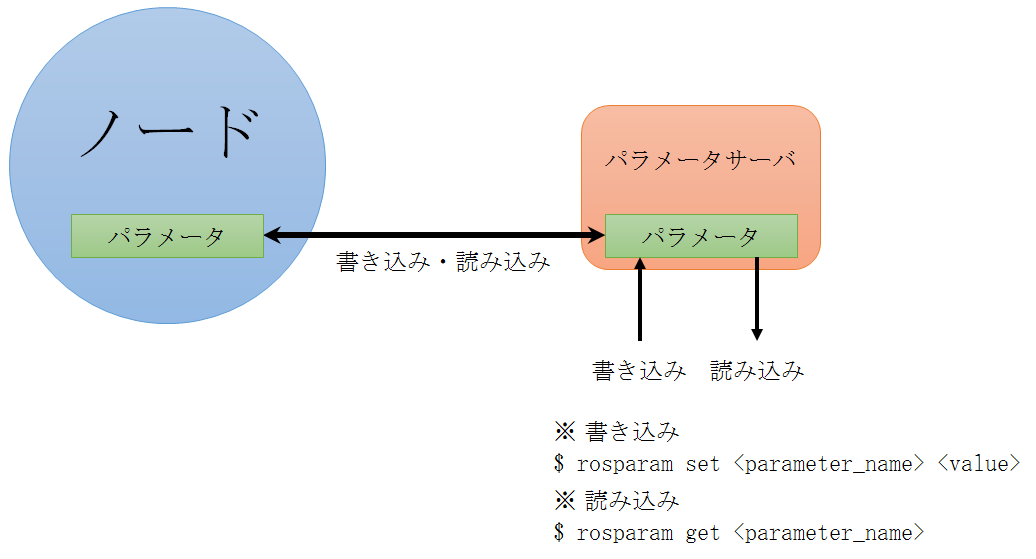
\includegraphics[width=10cm]{pictures/chapter6/pic_06_04.png}
  \caption{パラメータ通信}
\end{figure}

%-------------------------------------------------------------------------------
\section{トピック通信の実践}\index{トピック通信の実践}

トピック  通信では、送信側のノードを「Publisher(配信者)」、受信側のノードを「Subscriber(購読者)」と呼ぶ。本節では、メッセージファイルと配信者ノード、購読者ノードを含む簡単なパッケージを作成する  ことで、ROSにおけるトピックを用いた通信方式を理解する。

%-------------------------------------------------------------------------------
\subsection{パッケージの作成}

まず、irvs\_ros\_tutorialsという名前のパッケージを作成する。このパッケージでは、ROSの標準的なメッセージパッケージのstd\_msgsと、ROSでC/C++を使用する際に必要なクライアントライブラリroscppを使用する。このため、これをオプションで指定してcatkin\_create\_pkgを実行する。

\begin{lstlisting}[language=ROS]
$ cd ~/catkin_ws/src
$ catkin_create_pkg irvs_ros_tutorials std_msgs roscpp
\end{lstlisting}

std\_msgsやroscppなどのパッケージは、作成されたパッケージをビルドする前に、あらかじめインストールしておく必要がある。これら依存するパッケージやライブラリの設定は、上記のようにcatkin\_create\_pkgコマンドで新たにパッケージを作成するときに指定することもできるが、  作成した後にpackage.xmlを直接編集して指定することもできる。

パッケージを作成すると、「\verb|~|/catkin\_ws/src」フォルダにirvs\_ros\_tutorialsパッケージフォルダが作られ、その中に必要なROSのパッケージやCMakeLists.txt、 package.xmlファイルが置かれる。次のようにlsコマンドを入力するか、Nautilusを利用してパッケージのフォルダを確認すると、以下のように表示される。次項では、ここで作成されたpackage.xml、CMakeLists.txtを修正する。

\begin{lstlisting}[language=ROS]
$ cd irvs_ros_tutorials
$ ls
include     %*→ヘッダーファイルフォルダ*)
src     %*→ソースコードフォルダ*)
CMakeLists.txt    %*→ビルド設定ファイル*)
package.xml   %*→パッケージの設定ファイル*)
\end{lstlisting}

%-------------------------------------------------------------------------------
\subsection{パッケージの設定ファイル(package.xml)の修正}

ROSの必須の設定ファイルであるpackage.xmlは、パッケージ名、著作者、ライセンス、依存パッケージなどのパッケージの情報をXML形式で記述している。gedit、vim、emacsなどの文書編集プログラムでこのファイルを開き、現在のノードに合わせて内容を変更する。つぎのコマンドはUbuntu標準の文書編集プログラムgeditでpackage.xmlファイルを編集する例である。

\begin{lstlisting}[language=ROS]
$ gedit package.xml
\end{lstlisting}

以下のpackage.xmlファイルは、6.2.1項で作成したファイルを本節で作成するパッケージ  に合わせて変更した例である。  各オプションの詳細については、3.4.2項を参照してほしい。

ファイル名: package.xml
\begin{lstlisting}[language=XML]
<? xml version = "1.0" ?>
<package>
<name>irvs_ros_tutorials</name>
<version> 0.1.0 </version>
<description>The irvs_ros_tutorials package</description>
<maintainer email = "aaa@bbb.jp">Anonymous</maintainer>
<url type = "website"> http://irvs.github.io/ros_tms/</url>
<url type = "repository"> https://github.com/irvs/irvs_ros_tutorials.git </url>
<author email = "aaa@bbb.jp">Anonymous</author>

<license> BSD </license>

<buildtool_depend> catkin </buildtool_depend>

<build_depend> roscpp </build_depend>
<build_depend> std_msgs </build_depend>
<build_depend> message_generation </build_depend>

<run_depend> roscpp </run_depend>
<run_depend> std_msgs </run_depend>
<run_depend> message_runtime </run_depend>

<export>
</export>
</package>
\end{lstlisting}

%-------------------------------------------------------------------------------
\subsection{ビルド設定ファイル(CMakeLists.txt)の修正}

続いて同じフォルダのCMakeLists.txtファイルに、実行ファイルの作成、依存パッケージの優先ビルド、リンクの作成などを設定する。

\begin{lstlisting}[language=ROS]
$ gedit CMakeLists.txt
\end{lstlisting}

以下のCMakeLists.txtは、6.2.1項で作成したファイルを本節で作成するパッケージに合わせて変更したものである。前項のpackage.xmlファイルと同様に、各オプションの詳細については3.4.3項を参照してほしい。

ファイル名: CMakeLists.txt
\begin{lstlisting}[language=make]
cmake_minimum_required (VERSION 2.8.3)
project(irvs_ros_tutorials)

## %*catkinビルドに必要なコンポーネントパッケージの設定*)
## %*これらのパッケージが存在しない場合、catkinビルドの途中でエラーが出る。*)
find_package(catkin REQUIRED COMPONENTS roscpp std_msgs message_generation)

## %*メッセージファイルの設定*)
add_message_files(FILES msgTutorial.msg)

##  %*add\_message\_filesで使用するメッセージの依存関係を設定*)
## %*これらのパッケージが存在しない場合、catkinビルドの途中でエラーが出る。*)
generate_messages(DEPENDENCIES std_msgs)

## %*インクルードディレクトリ、ライブラリ、catkinビルド、システムに依存するパッケージの指定*)
catkin_package(
  INCLUDE_DIRS include
  LIBRARIES irvs_ros_tutorials
  CATKIN_DEPENDS roscpp std_msgs
  DEPENDS system_lib
)

## %*インクルードディレクトリの設定*)
include_directories(include ${catkin_INCLUDE_DIRS})

## %*ros\_tutorial\_msg\_publisherノードの設定*)
## %*実行ファイル、ターゲットリンクライブラリ、追加の依存関係などを設定*)
add_executable(ros_tutorial_msg_publisher
  src/ros_tutorial_msg_publisher.cpp)
target_link_libraries(ros_tutorial_msg_publisher ${catkin_LIBRARIES})
add_dependencies(ros_tutorial_msg_publisher
  irvs_ros_tutorials_generate_messages_cpp)

## %*ros\_tutorial\_msg\_subscriberノードの設定*)
## %*実行ファイル、ターゲットリンクライブラリ、追加の依存関係などを設定*)
add_executable(ros_tutorial_msg_subscriber
  src/ros_tutorial_msg_subscriber.cpp)
target_link_libraries(ros_tutorial_msg_subscriber ${catkin_LIBRARIES})
add_dependencies(ros_tutorial_msg_subscriber
  irvs_ros_tutorials_generate_messages_cpp)
\end{lstlisting}

%-------------------------------------------------------------------------------
\subsection{メッセージファイルの作成}

前項でCMakeLists.txtファイルには、次のようなオプションを追加した。

\begin{lstlisting}[language=make]
add_message_files(FILES msgTutorial.msg)
\end{lstlisting}

このオプションは、6.2.1項で作成したパッケージに含まれるノードでmsgTutorial.ms\\gメッセージを使用するため、そのメッセージ型を定義したmsgTutorial.hファイルを作成する ための設定である。ただしメッセージファイルmsgTutorial.msg自体はまだ作成していないので、次の手順で作成する。

\begin{lstlisting}[language=ROS]
$ roscd irvs_ros_tutorials  %*→パッケージフォルダに移動*)
$ mkdir msg    %* →パッケージにmsgフォルダを新規作成*)
$ cd msg      %*→作成したmsgフォルダに移動*)
$ gedit msgTutorial.msg %*→msgTutorial.msgファイルを新規作成する*)
\end{lstlisting}

メッセージ内容は以下の通りで、int32(32ビット整数型)メッセージ形式のdata変数を宣言している  。

\begin{lstlisting}[language=ROS]
int32 data
\end{lstlisting}

メッセージタイプはint32以外にもbool、int8、int16、float32、string、time、durationなどの基本的な形式   、およびactionlib\_msgsやdiagnostic\_msgsなど、ROSで多く使用されているメッセージをまとめたcommon\_msgsなどがある。ここでは、最も簡単な例としてint32を宣言した。

\begin{exercise}[メッセージ・サービスファイルの独立パッケージ化]
メッセージファイルmsgとサービスファイルsrvは、実行ノードパッケージに含めるのではなく、メッセージファイルだけで構成された独立したパッケージとすることを推奨する。購読者ノードと配信者ノードを別のコンピュータ上で実行するとき、その両方のノードには相互に依存関係があるので、片方のノードにしか関連しないパッケージやノードであっても、すべて双方のコンピュータに  インストールする必要がある。しかしメッセージのみの独立したパッケージを個別に作成しておけば、このパッケージのみを追加でインストールすればよく    、一方のノードだけに関連したパッケージを他方のノードを実行するコンピュータにインストールする必要がなくなる。ただし、本書では、コードを簡潔に示すため、メッセージファイルを実行ノードパッケージに含めている。
\end{exercise}

%-------------------------------------------------------------------------------
\subsection{配信者ノードの作成}

前述のCMakeLists.txtファイルには、次のような配信者  ノードの実行ファイルを生成するオプションを追加した。

\begin{lstlisting}[language=make]
add_executable(ros_tutorial_msg_publisher  src/ros_tutorial_msg_publisher.cpp)
\end{lstlisting}

これは、srcフォルダのros\_tutorial\_msg\_publisher.cppという名前のファイルから、ros\_tutorial\_msg\_publisherという実行ファイルを作成することを意味する。次の手順で配信者ノードのためのプログラムを作成してみよう。

\begin{lstlisting}[language=ROS]
$ roscd irvs_ros_tutorials/src %*→ パッケージのソースフォルダであるsrcフォルダに移動*)
$ gedit ros_tutorial_msg_publisher.cpp %*→ ソースファイルの新規作成と内容の変更*)
\end{lstlisting}

ファイル名: ros\_tutorial\_msg\_publisher.cpp
\begin{lstlisting}[language=C++]
// %*ROSメインヘッダーファイル*)
// %*ROSプログラミングを行う際に必要となるROSファイルのインクルードを行う。*)
// %*後述するROS\_INFO関数などを使用できるようになる。*)
#include "ros/ros.h"

// %*msgTutorialメッセージファイルのヘッダー*)
// %*CMakelists.txtでビルド後に自動的に生成されるように設定した*)
// %*メッセージファイルのヘッダーをインクルードする。*)
#include "irvs_ros_tutorials/msgTutorial.h"

// %*配信者ノードのメイン関数*)
int main(int argc, char **argv)
{
  // %*ノード名の初期化*)
  ros::init(argc, argv, "ros_tutorial_msg_publisher");
  // %*ROSシステムとの通信のためのノードハンドルを宣言*)
  ros::NodeHandle nh;

  // %*配信者ノードの宣言*)
  // %*irvs\_ros\_tutorialsパッケージのmsgTutorialメッセージファイルを*)
  // %*利用した配信者ros\_tutorial\_pubを宣言する。*)
  // %*トピック名を ros\_tutorial\_msg とし、配信者キュー( queue )の*)
  // %*サイズを100に設定する。*)
  // %*配信者キューには、メッセージを送る際、メッセージデータを蓄積する。*)
   // %*http://wiki.ros.org/msg*)
   ros::Publisher ros_tutorial_pub =
     nh.advertise<irvs_ros_tutorials::msgTutorial>("ros_tutorial_msg", 100);

   // %*ループの周期を設定する。 "10"は10Hzを表し、0.1秒間隔で繰り返される*)
   // %*http://wiki.ros.org/roscpp/Overview/Time*)
  ros::Rate loop_rate(10);

  // %*メッセージに使用する変数の宣言*)
  int count = 0;

  // %*ros::ok()はROSの動作が正常であるならtrueを返す関数である。*)
  while (ros::ok())
  {
    // %*msgTutorialメッセージファイル形式でmsg変数を宣言する。*)
    irvs_ros_tutorials::msgTutorial msg;

    // %*変数countを使用して、メッセージの値を定める。*)
    msg.data = count;

    // %*ROS\_INFOというROS関数を使用して、count変数を表示する。*)
    ROS_INFO("send msg = %d", count);

    // %*メッセージを発行する。約0.1秒間隔で発行される。*)
    ros_tutorial_pub.publish(msg);

    // %*上で定められたループサイクルになるように、スリープに入る*)
    loop_rate.sleep();

    // %*count変数に1ずつ増加*)
    ++count;
  }
  return 0;
}
\end{lstlisting}

%-------------------------------------------------------------------------------
\subsection{購読者ノードの作成}

CMakeLists.txtファイルには、次のような購読者 ノードの実行ファイルを生成するオプションを追加した。

\begin{lstlisting}[language=make]
add_executable(ros_tutorial_msg_subscriber src/ros_tutorial_msg_subscriber.cpp)
\end{lstlisting}

これは、srcフォルダのros\_tutorial\_msg\_subscriber.cppという名前のファイルから、ros\_tutorial\_msg\_subscriberという実行ファイルを作成することを意味する。次の手順で購読者ノードのためのプログラムを作成してみよう。

\begin{lstlisting}[language=ROS]
$ roscd irvs_ros_tutorials/src %*→ パッケージのソースフォルダであるsrcフォルダに移動*)
$ gedit ros_tutorial_msg_subscriber.cpp %*→ ソースファイルの新規作成と内容の変更*)
\end{lstlisting}

ファイル名: ros\_tutorial\_msg\_subscriber.cpp
\begin{lstlisting}[language=C++]
// %*ROSメインヘッダーファイル*)
// %*ROSプログラミングを行う際に必要となるROSファイルのインクルードを行う。*)
// %*後述するROS\_INFO関数などを使用できるようになる。*)
#include "ros/ros.h"

// %*msgTutorialメッセージファイルのヘッダー*)
// %*CMakelists.txtでビルド後に自動的に生成されるように設定した*)
// %*メッセージファ//イルのヘッダーをインクルードする。*)
#include "irvs_ros_tutorials/msgTutorial.h"

// %*メッセージを受信したときに動作するコールバック関数を定義*)
// %*irvs\_ros\_tutorialsパッケージのmsgTutorialメッセージを受信する*)
void msgCallback(const irvs_ros_tutorials::msgTutorial::ConstPtr& msg)
{
  // %*受信したメッセージを表示する。*)
  ROS_INFO("recieve msg: %d", msg->data);
}

// %*購読者ノードのメイン関数*)
int main(int argc, char **argv)
{
  // %*ノード名の初期化*)
  ros::init(argc, argv, "ros_tutorial_msg_subscriber");
  // %*ROSシステムとの通信のためのノードのハンドルを宣言*)
  ros::NodeHandle nh;

  // %*購読者ノードの宣言*)
  // %*irvs\_ros\_tutorialsパッケージのmsgTutorialメッセージファイルを*)
  // %*利用した購読者ros\_tutorial\_subを宣言する。*)
  // %*トピック名をros\_tutorial\_msg とし、購読者キュー( queue )の*)
  // %*サイズを100に設定する。*)
  // %*購読者キューには、配信者から送信されてくるメッセージが蓄積される。*)
  ros::Subscriber ros_tutorial_sub = nh.subscribe("ros_tutorial_msg",
   100, msgCallback);

  // %*メッセージが受信されるまで待機し、受信が行われた場合、*)
  // %*コールバック関数を実行する。*)
  ros::spin();

  return 0;
}
\end{lstlisting}

%-------------------------------------------------------------------------------
\subsection{ROSノードのビルド}

次のコマンドでirvs\_ros\_tutorialsパッケージのメッセージファイル、配信者ノード、購読者ノードをビルドする。

\begin{lstlisting}[language=ROS]
$ cd ~/catkin_ws  %*→ catkinフォルダに移動*)
$ catkin_make   %*→ catkinビルドを実行する*)
\end{lstlisting}

irvs\_ros\_tutorialsパッケージのプログラムは、「\verb|~|/catkin\_ws/src/irvs\_ros\_tutorials/src」フォルダにあり、irvs\_ros\_tutorialsパッケージのメッセージファイルは「\verb|~|/catkin\_ws/src\\/irvs\_ros\_tutorials/msg」フォルダにある。
このコマンドにより、「\verb|~|/catkin\_ws/build」と「\verb|~|/catkin\_ws /develフォルダにそれぞれファイルが生成される。「\verb|~|/catkin\_ws/build」フォルダには、catkinビルドで使用された設定内容が保存され、「\verb|~|/catkin\_ws/devel/lib/irvs\\\_ros\_tutorials」フォルダには実行ファイルが、「\verb|~|/catkin\_ws/devel/include/irvs\_ros\_tutorials\\」にはメッセージファイルから自動生成されたヘッダーファイルが保存される。

%-------------------------------------------------------------------------------
\subsection{配信者ノードの実行}

それでは、作成した配信者ノードを実行しよう。ノードの実行前にroscoreを実行して、マスターを起動する。

\begin{lstlisting}[language=ROS]
$ roscore
\end{lstlisting}

その後、別のターミナルウインドウを開き、ROSのノード実行コマンドであるrosrunを利用して、irvs\_ros\_tutorialsパッケージのros\_tutorial\_msg\_publisherノードを起動する。

\begin{lstlisting}[language=ROS]
$ rosrun irvs_ros_tutorials ros_tutorial_msg_publisher
\end{lstlisting}

配信者ノードを実行すると、図6-5のような出力画面が表示され、ROSメッセージが配信されているのがわかる。

\begin{figure}[h]
  \centering
  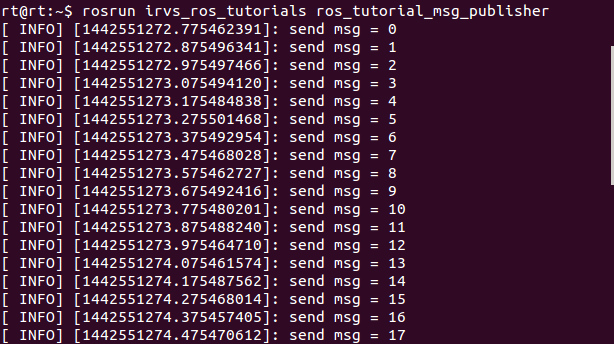
\includegraphics[width=10cm]{pictures/chapter6/pic_06_05.png}
  \caption{ros\_tutorial\_msg\_publisherノードの実行画面}
\end{figure}

4章で紹介したrostopicコマンドを実行して、ROSのネットワークで使用されているトピックのリストを確認してみよう。rostopicコマンドにlistオプションを付けて実行すると、ros\_tutorial\_msgトピックがあることを確認できる。

\begin{lstlisting}[language=ROS]
$ rostopic list
/ros_tutorial_msg
/rosout
/rosout_agg
\end{lstlisting}

次に、rostopicコマンドにechoオプションを付けて、ros\_tutorial\_msgトピックのメッセージの内容を表示すると、図6-6のように「data: 2」などの実際に配信されているトピックの内容が確認できる  。

\begin{lstlisting}[language=ROS]
$ rostopic echo /ros_tutorial_msg
\end{lstlisting}

\begin{figure}[h]
  \centering
  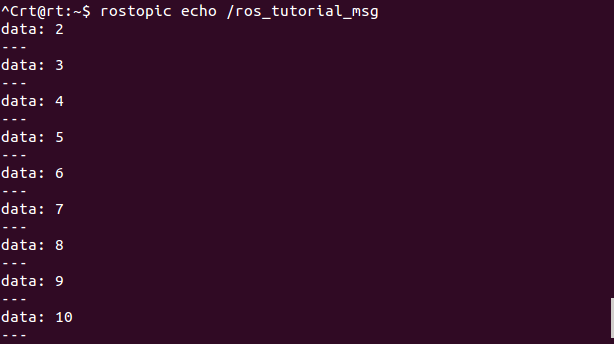
\includegraphics[width=10cm]{pictures/chapter6/pic_06_06.png}
  \caption{ros\_tutorial\_msgトピックの内容}
\end{figure}

%-------------------------------------------------------------------------------
\subsection{購読者ノードの実行}

配信者ノードを実行したまま、購読者ノードを実行する。新しいターミナルウインドウを開き、ROSのノード実行コマンドであるrosrunを利用して、irvs\_ros\_tutorialsパッケージのros\_tutorial\_msg\_subscriberノードを起動する。

\begin{lstlisting}[language=ROS]
$ rosrun irvs_ros_tutorials ros_tutorial_msg_subscriber
\end{lstlisting}

購読者ノードを実行すると、図6-7のような出力画面が表示される。配信者ノードから送信されたros\_tutorial\_msgトピックのメッセージを、購読者ノードが受信した結果が表示される。

\begin{figure}[h]
  \centering
  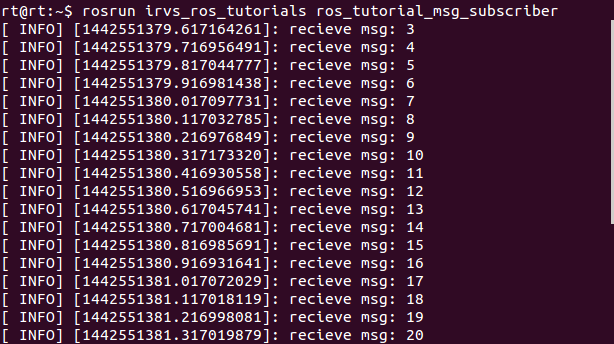
\includegraphics[width=10cm]{pictures/chapter6/pic_06_07.png}
  \caption{ros\_tutorial\_msg\_subscriberノードの実行画面}
\end{figure}


%-------------------------------------------------------------------------------
\subsection{実行ノードの通信状態の確認}

配信者および購読者ノードを実行したら、5.2節で紹介したrqtを利用して、実行中のノードの通信状態を確認してみよう。次のようにrqt\_graph、あるいはrqtのいずれかを実行する。

\begin{lstlisting}[language=ROS]
$ rqt_graph
\end{lstlisting}

\begin{lstlisting}[language=ROS]
$ rqt
\end{lstlisting}

rqt上のメニューの[Plugins]→[Introspection]→[Node Graph]を選択すれば、図6-8のように、現在ROSで実行しているノードとメッセージが確認できる。

\begin{figure}[h]
  \centering
  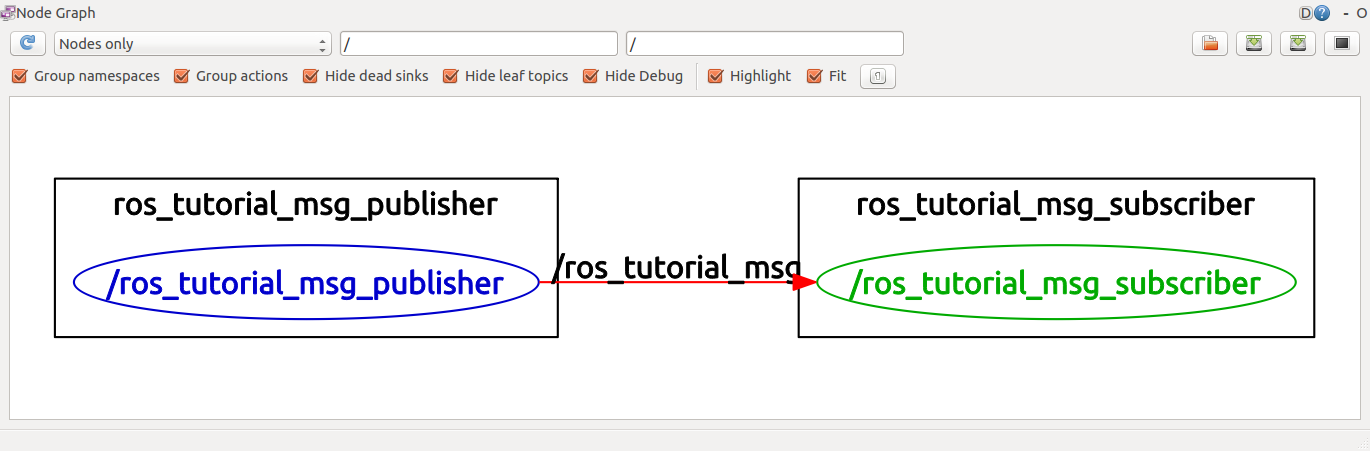
\includegraphics[width=10cm]{pictures/chapter6/pic_06_08.png}
  \caption{ノードの関係をrqt上で表示した結果}
\end{figure}

図6-8では、現在のROSネットワーク上には、配信者ノード(ros\_tutorial\_msg\_publish\\er)がトピック(ros\_tutorial\_msg)を配信しており、これを購読者ノード(ros\_tutorial\_msg\_\\subscriber)が受信していることが確認できる。

%-------------------------------------------------------------------------------
\section{サービス通信の実践}\index{サービス通信の実践}

本節では、単純なサービス·ファイルとサービスサーバ(server)ノード、サービスクライアント(client)ノードを作成する。前節で既にirvs\_ros\_tutorialsという名前のパッケージを作成したので、これを利用する。6.2.1項で行ったpackage.xmlファイルの修正は、ここでは必要ないので省略する。

%-------------------------------------------------------------------------------
\subsection{ビルド設定ファイル(CMakeLists.txt)の修正}

前節で作成したirvs\_ros\_tutorialsパッケージに、新しいサービスサーバノード、クライアントノード、サービスファイル(*.srv)を追加する。まず、次のようにirvs\_ros\_tutorial\\sパッケージに移動した後、CMakeLists.txtファイルを変更する。

\begin{lstlisting}[language=ROS]
$ roscd irvs_ros_tutorials
$ gedit CMakeLists.txt
\end{lstlisting}

以下のCMakeLists.txtは、6.2.3項で作成したファイルを本節で作成するパッケージに合わせて変更したものである。前節のパッケージに、サービスサーバノードとクライアントノード、サービスファイル(*.srv)の内容を追加した(太字)。各オプションの詳細については、3.4.3項を参照してほしい。

ファイル名: CMakeLists.txt
\begin{lstlisting}[language=make]
cmake_minimum_required(VERSION 2.8.3)
project(irvs_ros_tutorials)

## %*catkinビルドに必要なコンポーネントパッケージの設定*)
## %*これらのパッケージが存在しない場合、catkinビルドの途中でエラーが出る。*)
find_package(catkin REQUIRED COMPONENTS roscpp std_msgs message_generation)

## %*メッセージファイルの設定*)
add_message_files(FILES msgTutorial.msg)

## %*サービスファイルの設定*)
add_service_files(FILES srvTutorial.srv)

## %*add\_message\_filesで使用するメッセージの依存関係を設定*)
## %*これらのパッケージが存在しない場合、catkinビルドの途中でエラーが出る。*)
generate_messages(DEPENDENCIES std_msgs)

## %*インクルードディレクトリ、ライブラリ、catkinビルド、システムに依存するパッケージの指定*)
catkin_package(
  INCLUDE_DIRS include
  LIBRARIES irvs_ros_tutorials
  CATKIN_DEPENDS roscpp std_msgs
  DEPENDS system_lib
)

## %*インクルードディレクトリの設定*)
include_directories(include ${catkin_INCLUDE_DIRS})

## %*ros\_tutorial\_msg\_publisherノードの設定*)
##  %*実行ファイル、ターゲットリンクライブラリ、追加の依存関係などを設定*)
add_executable(ros_tutorial_msg_publisher
  src/ros_tutorial_msg_publisher.cpp)
target_link_libraries(ros_tutorial_msg_publisher ${catkin_LIBRARIES})
add_dependencies(ros_tutorial_msg_publisher
  irvs_ros_tutorials_generate_messages_cpp)

## %*ros\_tutorial\_msg\_subscriberノードの設定*)
## %*実行ファイル、ターゲットリンクライブラリ、追加の依存関係などを設定*)
add_executable(ros_tutorial_msg_subscriber
  src/ros_tutorial_msg_subscriber.cpp)
target_link_libraries(ros_tutorial_msg_subscriber ${catkin_LIBRARIES})
add_dependencies(ros_tutorial_msg_subscriber
  irvs_ros_tutorials_generate_messages_cpp)

## %*ros\_tutorial\_srv\_serverサービスサーバノードの設定*)
## %*実行ファイル、ターゲットリンクライブラリ、追加の依存関係などを設定*)
add_executable(ros_tutorial_srv_server src/ros_tutorial_srv_server.cpp)
target_link_libraries(ros_tutorial_srv_server ${catkin_LIBRARIES})
add_dependencies(ros_tutorial_srv_server
  irvs_ros_tutorials_generate_messages_cpp)

## %*ros\_tutorial\_srv\_clientサービスクライアントノードの設定*)
## %*実行ファイル、ターゲットリンクライブラリ、追加の依存関係などを設定*)
add_executable(ros_tutorial_srv_client src/ros_tutorial_srv_client.cpp)
target_link_libraries(ros_tutorial_srv_client ${catkin_LIBRARIES})
add_dependencies(ros_tutorial_srv_client
  irvs_ros_tutorials_generate_messages_cpp)
\end{lstlisting}

%-------------------------------------------------------------------------------
\subsection{サービスファイルの作成}

前項でCMakeLists.txtファイルには、次のようなオプションを追加した。

\begin{lstlisting}[language=make]
add_service_files(FILES srvTutorial.srv)
\end{lstlisting}

このオプションは、6.2.1項で作成したパッケージに含まれるノードでmsgTutorial.sr\\vサービスを使用するため、そのメッセージ型を定義したmsgTutorial.hファイルを作成する ための設定である 。ただしサービスファイルmsgTutorial.srv自体はまだ作成していないので、次の手順で作成する。

\begin{lstlisting}[language=ROS]
$ roscd irvs_ros_tutorials  %*→ パッケージフォルダに移動*)
$ mkdir srv     %*→ パッケージにsrvフォルダを新規作成*)
$ cd srv      %*→ 作成したsrvフォルダに移動*)
$ gedit srvTutorial.srv %*→ srvTutorial.srvファイルを新規作成する*)
\end{lstlisting}

サービス内容は以下の通りで、int64(64ビット整数型)メッセージ形式のサービスリクエスト(request)であるa、b変数と、サービスレスポンス(response)であるresult  変数を宣言している。 なお、「---」は、リクエストとレスポンスを区別するセパレータである。

ファイル名: srvTutorial.srv
\begin{lstlisting}[language=ROS]
int64 a
int64 b
---
int64 result
\end{lstlisting}

%-------------------------------------------------------------------------------
\subsection{サービスサーバノードの作成}

前述のCMakeLists.txtファイルには、次のようなサービスサーバノードの実行ファイルを生成するオプションを追加した。

\begin{lstlisting}[language=make]
add_executable(ros_tutorial_srv_server src/ros_tutorial_srv_server.cpp)
\end{lstlisting}

これは、srcフォルダのros\_tuto\\rial\_srv\_server.cppという名前のファイルから、 ros\_tutorial\_srv\_serverという実行ファイルを作成することを意味する。
次の手順でサービスサーバノードのためのプログラムを作成してみよう。

\begin{lstlisting}[language=ROS]
$ roscd irvs_ros_tutorials/src %*→ パッケージのソースフォルダであるsrcフォルダに移動*)
$ gedit ros_tutorial_srv_server.cpp %*→ ソースファイルの新規作成と内容の変更*)
\end{lstlisting}

ファイル名: ros\_tutorial\_srv\_server.cpp
\begin{lstlisting}[language=C++]
// %*ROSメインヘッダーファイル*)
// %*ROSプログラミングを行う際に必要となるROSファイルのインクルードを行う。*)
// %*後述するROS\_INFO関数などを使用できるようになる。*)
#include "ros/ros.h"

// %*srvTutorial サービスファイルのヘッダー*)
// %*CMakelists.txtでビルド後に自動的に生成されるように設定した*)
// %*サービスファイルのヘッダーをインクルードする。*)
#include "irvs_ros_tutorials/srvTutorial.h"

// %*サービスリクエストがある場合は、以下の処理を実行する。*)
// %*サービスリクエストは、req、サービスのレスポンスは、resに設定した。*)
bool calculation(irvs_ros_tutorials::srvTutorial::Request &req,
                 irvs_ros_tutorials::srvTutorial::Response &res)
{
  // %*サービスリクエストで受けたaとbの値を加えて、*)
  // %*サービスのレスポンス値に格納する。*)
  res.result = req.a + req.b;

  // %*サービスリクエストで受けたa、bの値の表示、および*)
  // %*サービスレスポンスに対応するresultの値を出力する。*)
  ROS_INFO("request: x=%ld, y=%ld", (long int)req.a, (long int)req.b);
  ROS_INFO("sending back response: [%ld]", (long int)res.result);
  return true;
}

// %*サービスサーバノードのメイン関数*)
int main(int argc, char **argv)
{
  // %*ノード名の初期化*)
  ros::init(argc, argv, "ros_tutorial_srv_server");
  // %*ROSシステムとの通信のためのノードのハンドルを宣言*)
  ros::NodeHandle nh;

  // %*サービスサーバ宣言*)
  // %*irvs\_ros\_tutorialsパッケージのsrvTutorialサービスファイルを利用した*)
  // %*サービスサーバros\_tutorial\_service\_serverを作成する。*)
  // %*サービス名はros\_tutorial\_srvで、サービスリクエストがあったとき、*)
  // %*calculationという関数を実行するように設定している。*)
  ros::ServiceServer ros_tutorial_service_server =
   nh.advertiseService("ros_tutorial_srv",calculation);

  // %*サービスサーバが実行したことを表示する。*)
  ROS_INFO("ready srv server!");

  // %*サービスリクエストを待機する*)
  ros::spin();

  return 0;
}
\end{lstlisting}

%-------------------------------------------------------------------------------
\subsection{サービスクライアントノードの作成}

CMakeLists.txtファイルには、次のようなサービスクライアントノードの実行ファイルを生成するオプションを追加した。

\begin{lstlisting}[language=make]
add_executable(ros_tutorial_srv_client src/ros_tutorial_srv_client.cpp)
\end{lstlisting}

これは、srcフォルダのros\_tuto\\rial\_srv\_client.cppという名前のファイルから、ros\_tutorial\_srv\_clientという実行ファイルを作成することを意味する。
 次の手順で  サービスクライアントノードのためのプログラムを作成してみよう。

\begin{lstlisting}[language=ROS]
$ roscd irvs_ros_tutorials/src %*→ パッケージのソースフォルダであるsrcフォルダに移動*)
$ gedit ros_tutorial_srv_client.cpp %*→ ソースファイルの新規作成と内容の変更*)
\end{lstlisting}

ファイル名: ros\_tutorial\_srv\_client.cpp
\begin{lstlisting}[language=C++]
// %*ROSメインヘッダーファイル*)
// %*ROSプログラミングを行う際に必要となるROSファイルのインクルードを行う。*)
// %*後述するROS\_INFO関数などを使用できるようになる。*)
#include "ros/ros.h"

// %*srvTutorialサービスファイルのヘッダー*)
// %*CMakelists.txtでビルド後に自動的に生成されるように設定したサービスファ*)
// %*イルのヘッダーをインクルードする。*)
#include "irvs_ros_tutorials/srvTutorial.h"

// %*atoll関数を使用するためのライブラリ*)
#include <cstdlib>

// %*サービスクライアントノードのメイン関数*)
int main (int argc, char **argv)
{
  // %*ノード名の初期化*)
  ros::init(argc, argv, "ros_tutorial_srv_client");

  // %*入力値エラー処理*)
  if(argc !=  3)
  {
    ROS_INFO("cmd: rosrun ros_tutorial ros_tutorial_service_client arg0 arg1");
    ROS_INFO( "arg0: double number, arg1: double number");
    return 1;
  }

  // %*ROSシステムとの通信のためのノードのハンドル宣言*)
  ros::NodeHandle nh;

  // %*サービスクライアント宣言、*)
  // %*irvs\_ros\tutorialsパッケージのsrvTutorialサービスファイルを利用した。*)
  // %*サービスクライアントros\_tutorial\_service\_clientを作成する。*)
  // %*サービス名は「ros\_tutorial\_srv」である。*)
  ros::ServiceClient ros_tutorial_service_client =
   nh.serviceClient <irvs_ros_tutorials::srvTutorial>("ros_tutorial_srv");

  // %*srvという名前でsrvTutorialサービス  を利用する*)
  // %*サービスのファイルを宣言する。*)
  irvs_ros_tutorials::srvTutorial srv;

  // %*サービスリクエスト値をそれぞれのa、bに格納する。*)
  srv.request.a = atoll(argv [1]);
  srv.request.b = atoll(argv [2]);

  // %*サービスをリクエストし、レスポンスが返された場合、*)
  // %*レスポンス値を表示する。*)
  if(ros_tutorial_service_client.call(srv))
  {
    ROS_INFO("send srv request.a and b: %ld, %ld",
      (long int)srv.request.a, (long int)srv.request.b);
    ROS_INFO("receive srv.response.result: %ld",
      (long int)srv.response.result);
  }
  else
  {
    ROS_ERROR("Failed to call service ros_tutorial_srv");
    return 1;
  }
  return 0;
}
\end{lstlisting}

%-------------------------------------------------------------------------------
\subsection{ROSノードのビルド}

次のコマンドでirvs\_ros\_tutorialsパッケージのサービスファイル 、サービスサーバノードとクライアント·ノードをビルドする  。

\begin{lstlisting}[language=ROS]
$ cd ~/catkin_ws
$ catkin_make
\end{lstlisting}

irvs\_ros\_tutorialsパッケージのプログラムは、「\verb|~|/catkin\_ws/src/irvs\_ros\_tutorials/src」フォルダにあり、irvs\_ros\_tutorialsパッケージのサービスファイルは「\verb|~|/catkin\_ws/src /irvs\_ros\_tutorials/srv」フォルダにある。
このコマンドにより、「\verb|~|/catkin\_ws/build」と「\verb|~|/catkin\_ws /develフォルダにそれぞれファイルが生成される。「\verb|~|/catkin\_ws/build」フォルダには、catkinビルドで使用された設定内容が保存され、「\verb|~|/catkin\_ws/devel/lib/irvs\\\_ros\_tutorials」フォルダには実行ファイルが、「\verb|~|/catkin\_ws/devel/include/irvs\_ros\_tutorials\\」にはサービスファイルから自動的に生成されたヘッダーファイルが保存される。

%-------------------------------------------------------------------------------
\subsection{サービスサーバ  ノードの実行}

それでは、作成したサービスサーバノードを実行しよう。ノードの実行前に、roscore以外のターミナルウインドウを閉じておく。次に、新たなターミナルウインドウを開き、ROSのノード実行コマンドであるrosrunを利用して、irvs\_ros\_tutorialsパッケージのros\_tutorial\_srv\_serverノードを実行する。

\begin{lstlisting}[language=ROS]
$ rosrun irvs_ros_tutorials ros_tutorial_srv_server
[INFO] [1423118250.6704810023]: ready srv server !
\end{lstlisting}

これにより、サービスサーバノードはサービスリクエストが送られるまで待機する。

%-------------------------------------------------------------------------------
\subsection{サービスクライアントノード  の実行}

サービスサーバノードを実行したまま、サービスクライアントノードを実行する。新しいターミナルウインドウを開き、ROSのノード実行コマンドであるrosrunを利用して、irvs\_ros\_tutorialsパッケージのros\_tutorial\_srv\_clientノードを起動する。ただし、ここでは実行パラメータとして、引数2、3を与えた。

\begin{lstlisting}[language=ROS]
$ rosrun irvs_ros_tutorials ros_tutorial_srv_client 2 3
[INFO] [1423118255.156345643]: send srv.Request.a and b: 2, 3
[INFO] [1423118255.156345021]: receive srv.Response.result: 5
\end{lstlisting}

サービスクライアントを実行して、入力した実行パラメータ2と3をそれぞれサービスリクエスト値aとbとして送信する。その結果、レスポンス値としてaとbの和の5が返されている。ここでは、単純に和を求めるためのパラメータとしてサービスメッセージを利用したが、サービスメッセージによりノードの設定や処理を変更するなど、より複雑な処理にも使用できる  。

なお、サービスはトピックと異なり一回限りの通信であるため、6.2.10項と同様にrqt\_graphを実行しても、rqt\_graphには図6-9のように配信者と購読者ノード、トピックのみ表示され、サービスは表示されない。

\begin{figure}[h]
  \centering
  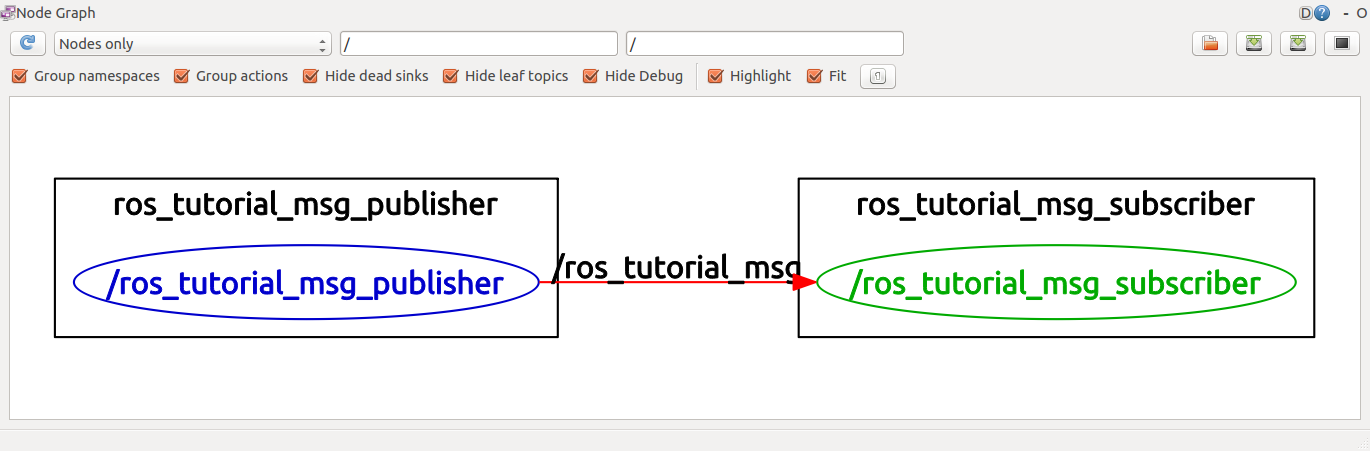
\includegraphics[width=12cm]{pictures/chapter6/pic_06_09.png}
  \caption{rqt上ではサービスは表示されない}
\end{figure}

%-------------------------------------------------------------------------------
\subsection{rosservice callコマンドを使用する方法}

サービスリクエストの実行は、6.3.7項のようにサービスクライアントノードを実行する方法以外にも、「rosservice call」というコマンドやrqtのServiceCallerを利用する方法もある。ここでは、「rosservice call」の使用例を示す。

\begin{lstlisting}[language=ROS]
$ rosservice call /ros_tutorial_srv 3 4
result: 7
\end{lstlisting}

「rosservice call」コマンドの後に「/ros\_tutorial\_srv」など、対応するサービス名を書き、その後にサービスリクエストに必要な実行パラメータを書く。ここでは、6.3.2項で示したように、サービスリクエスト値にint64型のaとbを設定しているので、実行パラメータとして3と4を入力した。これに対するサービスレスポンス値であるresultには、int64型の7が返されている。

%-------------------------------------------------------------------------------
\subsection{rqtのService Callerを使用する方法}

6.3.8項で説明した「rosservice call」は、ターミナルから直接実行できる利点があるが、LinuxやROSコマンドを使用に慣れていない場合にはrqtの「Service Caller」の使用が便利である。
サービスリクエストの実行に、GUI形式のインターフェースであるrqtの「Service Caller」を利用した例を示す。まず、ROSのGUIツールであるrqtを起動する。

\begin{lstlisting}[language=ROS]
$ rqt
\end{lstlisting}

次に、rqtプログラムのメニューから[Plugins]→[Service]→[Service Caller]を選択すると、図6-10のような画面が現れる。

\begin{figure}[h]
  \centering
  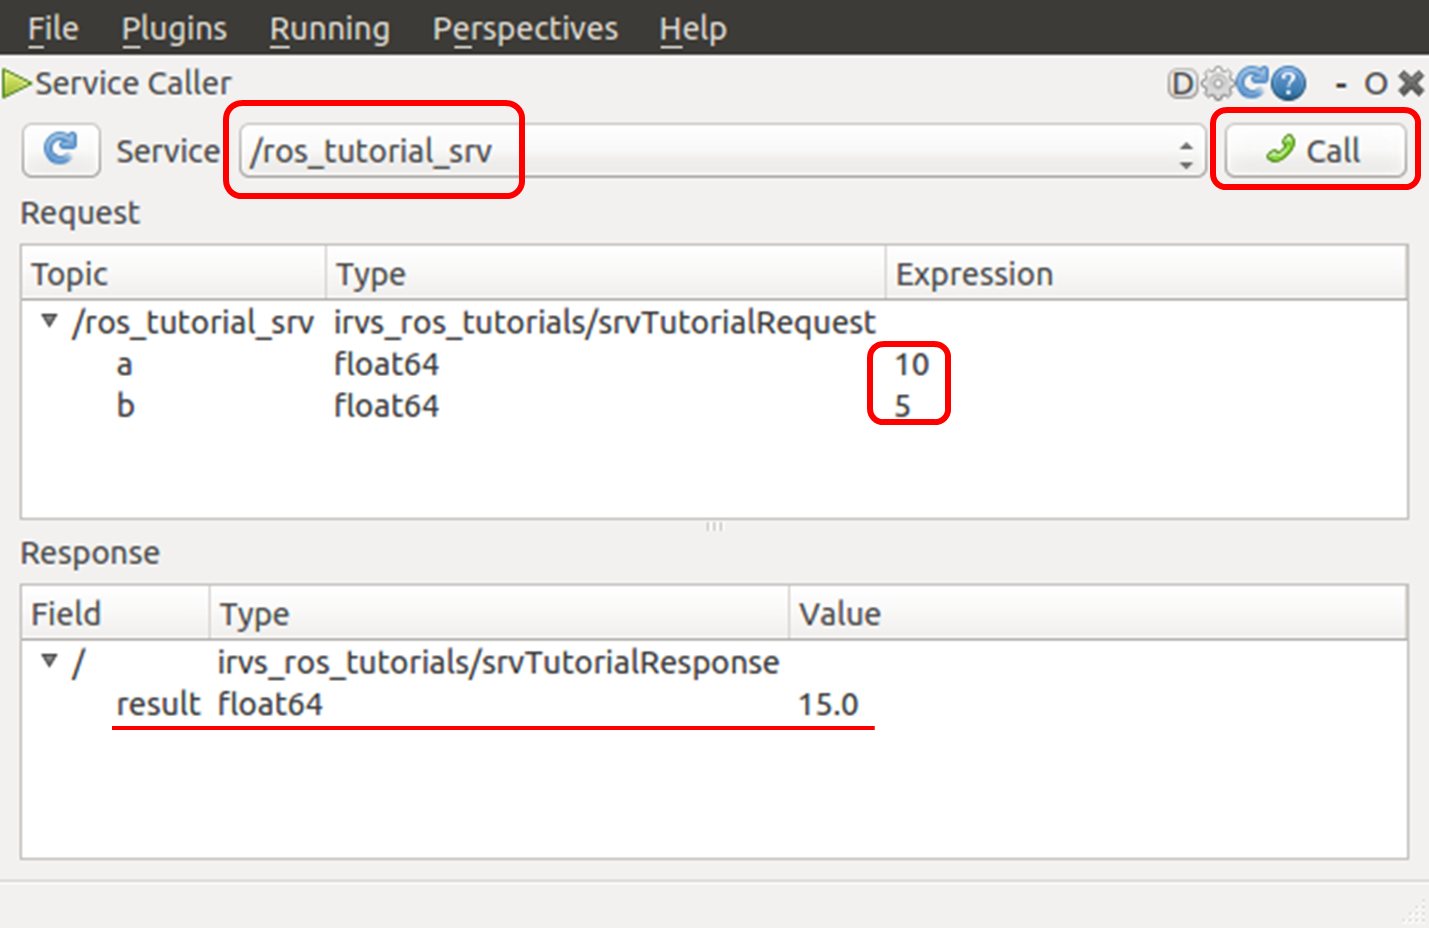
\includegraphics[width=12cm]{pictures/chapter6/pic_06_10.png}
  \caption{rqtのService Callerプラグインを使用したサービスリクエスト}
\end{figure}

画面上部にあるService欄でサービス名を選択すると、Request欄にサービスリクエストに必要な情報が表示されるので、それぞれのExpression欄に情報を入力する。この例では、aに10、bに5を入力した。次に、右上にある緑の電話の形の<Call>アイコンをクリックすると、サービスリクエストが実行され、Response欄にサービスレスポンス値が表示される。

本節では、サービスサーバノードとサービスクライアントノードを作成し、これらを実行して、ノード間でサービスを通信する方法について学んだ。関連するプログラムはhttps://github.com/irvs/irvs\_ros\_tutorialsから入手できる。すぐにプログラムを実行したい場合は、次のように「\verb|~|/catkin\_ws/src」フォルダから次のコマンドを実行すればよい。

\begin{lstlisting}[language=ROS]
$ cd ~/catkin_ws/src
$ git clone https://github.com/irvs/irvs_ros_tutorials.git
$ cd ~/catkin_ws
$ catkin_make
\end{lstlisting}

%-------------------------------------------------------------------------------
\section{パラメータ通信の実践}\index{パラメータ通信の実践}

本節では、パラメータの使用方法を、実例を交えて説明する。

%-------------------------------------------------------------------------------
\subsection{パラメータを利用したノードの作成}

6.3節で作成したサービスサーバノードros\_tutorial\_srv\_server.cpp  のプログラムを変更して、パラメータを利用してサービスリクエストに入力されたaとbの四則演算を行うノードを作成する。ros\_tutorial\_srv\_server.cppプログラムを変更する手順を以下に示す。

\begin{lstlisting}[language=ROS]
$ roscd irvs_ros_tutorials/src %*→ パッケージのソースコードフォルダのsrcフォルダに移動*)
$ gedit ros_tutorial_srv_server.cpp %*→ ソースファイルの内容の変更*)
\end{lstlisting}

ファイル名: ros\_tutorial\_srv\_server.cpp
\begin{lstlisting}[language=C++]
// %*ROSメインヘッダーファイル*)
// %*ROSプログラミングを行う際に必要となるROSファイルのインクルードを行う。*)
// %*後述するROS\_INFO関数などを使用できるようになる。*)
#include "ros/ros.h"

// %*srvTutorial サービスファイルのヘッダー*)
// %*CMakelists.txtでビルド後に自動的に生成されるように設定したサービスファ*)
// %*イルのヘッダーをインクルードする。*)
#include "irvs_ros_tutorials/srvTutorial.h"

// %*パラメータのオプション*)
#define PLUS  1  // %*加算*)
#define MINUS  2  // %*減算*)
#define MULTIPLICATION  3  // %*乗算*)
#define DIVISION  4  // %*割算*)

int g_operator = PLUS;

// %*サービスリクエストがある場合は、以下の処理を実行する。*)
// %*サービスリクエストは、req、サービスのレスポンスは、resに設定した。*)
bool calculation(irvs_ros_tutorials::srvTutorial::Request  &req,
                 irvs_ros_tutorials::srvTutorial::Response &res)
{
  // %*パラメータ値に基づいて演算子を変更し、サービスリクエストを受けた*)
  // %*aとbの値を計算して、結果をサービスレスポンス値に保存する  。*)
  switch(g_operator){
    case PLUS:
         res.result = req.a + req.b; break;
    case MINUS:
         res.result = req.a - req.b; break;
    case MULTIPLICATION:
         res.result = req.a * req.b; break;
    case DIVISION:
         if(req.b == 0){
           res.result = 0; break;
         }
         else{
           res.result = req.a / req.b; break;
         }
    default:
         res.result = req.a + req.b; break;
  }

  // %*サービスリクエストで受けたa、bの値の表示、および*)
  // %*サービスレスポンスに対応するresultの値を出力する。*)
  ROS_INFO("request: x=%ld, y=%ld", (long int)req.a, (long int)req.b);
  ROS_INFO("sending back response: [%ld]", (long int)res.result);

  return true;
}

// %*サービスサーバノードのメイン関数*)
int main(int argc, char **argv)
{
  // %*ノード名の初期化*)
  ros::init(argc, argv, "ros_tutorial_srv_server");
  // %*ROSシステムとの通信のためのノードのハンドルを宣言*)
  ros::NodeHandle nh;

  // %*ROSシステムとの通信のためのノードのハンドルを宣言(Private)*)
  // %*http://wiki.ros.org/Names*)
  ros::NodeHandle nh_priv("~");

  // %*パラメータの初期設定, http://wiki.ros.org/rosparam*)
  nh_priv.setParam("calculation_method", PLUS);

  // %*サービスサーバ宣言、*)
  // %*irvs\_ros\_tutorialsパッケージのsrvTutorialサービスファイルを利用した*)
  // %*サービスサーバros\_tutorial\_service\_serverを作成する。*)
  // %*サービス名はros\_tutorial\_srvで、サービスリクエストがあったとき、*)
  // %*calculationという関数を実行するように設定している。*)
  ros::ServiceServer ros_tutorial_service_server =
   nh.advertiseService("ros_tutorial_srv", calculation);

  // %*サービスサーバが実行したことを表示する。*)
  ROS_INFO("ready srv server!");

  // %*ループの周期を設定する。 "10"は10Hzを表し、*)
  // %*0.1秒間隔で繰り返される*)
  ros::Rate r(10);

  while (ros::ok())
  {
    // %*演算子をパラメータから取得した値に変更する。*)
    nh_priv.getParam("calculation_method", g_operator);

    // %*コールバック関数の処理ルーチン*)
    ros::spinOnce();

    // %*上で定められたループサイクルになるように、スリープに入る*)
    r.sleep();
  }
  return 0;
}
\end{lstlisting}

大部分は、6.3.3項で  作成した内容と同じだが、新たに追加した部分について見ていこう。特に、太字で表示した「setParam」と「getParam」がパラメータ処理を行う箇所で重要なので、以下で詳しく説明する。

%-------------------------------------------------------------------------------
\subsection{パラメータの設定}

6.4.1項のプログラムの最初の太字の部分では、  calculation\_methodという名前のパラメータをPLUSに設定している。

\begin{lstlisting}[language=C++]
nh.setParam("calculation_method", PLUS);
\end{lstlisting}

PLUSは、6.4.1項のプログラムの冒頭で1と定義したので、calculation\_methodのパラメータは1(=加算)になり、サービスリクエストで受信した値を加算して、その答えをサービスのレスポンスとして返す。

%-------------------------------------------------------------------------------
\subsection{パラメータの読み出し}

6.4.1項のプログラムの2つ目の太字の部分では、calculation\_methodという名前のパラメータをパラメータサーバから読み出してg\_operatorに値を代入している。

\begin{lstlisting}[language=C++]
nh.getParam("calculation_method", g_operator);
\end{lstlisting}

6.4.1項のプログラムでは、0.1秒ごとに以下の命令を実行し、パラメータの値をg\_operatorに代入している。

%-------------------------------------------------------------------------------
\subsection{ノードの作成と実行}

次のコマンドでirvs\_ros\_tutorialsパッケージのサービスサーバノードを構築する。

\begin{lstlisting}[language=ROS]
$ cd ~/catkin_ws
$ catkin_make
\end{lstlisting}

次のコマンドを実行すると、サービスサーバノードはサービスリクエストが送られるまで待機する。

\begin{lstlisting}[language=ROS]
$ rosrun irvs_ros_tutorials ros_tutorial_srv_server
[INFO] [1423133839.188884351]: ready srv server !
\end{lstlisting}

%-------------------------------------------------------------------------------
\subsection{パラメータのリストを表示}
次の「rosparam list」コマンドで、現在ROSネットワークで使用されているパラメータを確認できる。

\begin{lstlisting}[language=ROS]
$ rosparam list
/calculation_method
/rosdistro
/rosversion
/run_id
...
\end{lstlisting}

出力されたリストの中の「/calculation\_method」が、本節で使用するパラメータである。

%-------------------------------------------------------------------------------
\subsection{パラメータの使用例}

パラメータの値を変更するには「rosparam set」コマンドを用いる。以下のようにパラメータを変更して、同じサービスリクエストを実行してみよう  。

\begin{lstlisting}[language=ROS]
$ rosservice call /ros_tutorial_srv 10 5  %*→ 四則演算の変数a、bを入力*)
result: 15         %*→ デフォルトの加算*)
$ rosparam set /calculation_method 2    %*→ パラメータを減算に変更*)
$ rosservice call /ros_tutorial_srv 10 5
result: 5
$ rosparam set /calculation_method 3   %* → パラメータを乗算に変更*)
$ rosservice call /ros_tutorial_srv 10 5
result: 50
$ rosparam set /calculation_method 4   %* → パラメータを除算に変更*)
$ rosservice call /ros_tutorial_srv 10 5
result: 2
\end{lstlisting}

パラメータを変更すると、同一のサービスリクエストである「rosservice call /ros\_tutorial\_srv 10 5」を入力したにもかかわらず、結果(result)が異なることが確認できる。このようにパラメータを用いる  と、ユーザ側 からノードの設定や処理を変更できる。

%-------------------------------------------------------------------------------
\section{roslaunchを用いた複数ノードの起動}\index{roslaunchを用いた複数ノードの起動}

rosrunが一つのノードを実行するコマンドであるのに対し、roslaunchは、複数のノードを実行するコマンドである。またオプションにより、ノードの実行時のパラメータの変更、ノード名の変更、ノードの名前空間  (後述)の設定、ROS\_ROOTとROS\_PACK\\AGE\_PATHの設定、環境変数の変更なども可能である。
roslaunchは、「*.launch」というXML形式のファイルにより実行ノードを設定する。実行コマンドは、「roslaunch [パッケージ名] [roslaunchファイル]」である。
本節では、roslaunchを用いて、これまでに作成したros\_tutorial\_msg\_publisherとros\_tutorial\_msg\_subscriberノードを実行する例を示す。ただしROSネットワーク内ではノード名は重複してはならないため、発信者ノードと購読者ノードをそれぞれ2つずつ、名前を変えて起動して、お互い別々のメッセージ通信を行うことにする。

%-------------------------------------------------------------------------------
\subsection{roslaunchファイルの作成}

 roslaunchを利用するには、まず、パッケージフォルダにlaunchという名前のフォルダを作成し、その中に「*.launch」というファイルを作成する必要がある。次のコマンドでフォルダを作成し、ここではunion.launchという新しいファイルを作成する。

\begin{lstlisting}[language=ROS]
$ roscd irvs_ros_tutorials
$ mkdir launch
$ cd launch
$ gedit union.launch
\end{lstlisting}

union.launchファイルは、次のように設定する。

\begin{lstlisting}[language=XML]
union.launch
<launch>
<node pkg = "irvs_ros_tutorials" type = "ros_tutorial_msg_publisher" name = "msg_publisher1" />
<node pkg = "irvs_ros_tutorials" type = "ros_tutorial_msg_subscriber" name = "msg_subscriber1" />
<node pkg = "irvs_ros_tutorials" type = "ros_tutorial_msg_publisher" name = "msg_publisher2" />
<node pkg = "irvs_ros_tutorials" type = "ros_tutorial_msg_subscriber" name = "msg_subscriber2" />
</launch>
\end{lstlisting}

<launch>タグの間には、roslaunchコマンドでノードを実行するのに必要なタグを記述する。 <node>タグでは、roslaunchで実行するノードを記述し、オプションとして、pkg、type、nameを指定する。

\begin{itemize}
\item  pkg: パッケージの名前
\item type: 実行するノードの名前(ノード名)
\item name:  typeに設定されたノードが実行されるときに付けられる名前(実行名)。通常はtypeと同じ名前を設定するが、typeで指定したノード名が他のノードと重複する  場合は実行名を変更する。
\end{itemize}

%-------------------------------------------------------------------------------
\subsection{roslaunchによる複数のノードの実行}

roslaunchファイルを作成したら、roslaunchコマンドを用いて  union.launchを実行しよう。まず、roscore以外のターミナルウインドウを閉じる。次に、新たなターミナルウインドウを開き、次のように  roslaunchコマンドでunion.launchを実行する。

\begin{lstlisting}[language=ROS]
$ roslaunch irvs_ros_tutorials union.launch --screen
\end{lstlisting}

なお、roslaunchコマンドで複数のノードを実行するとき、実行されるノードの出力(info、errorなど)がターミナルウインドウに表示されないと、ノードの動作がわからずデバッグしにくい。この場合、「--screen」オプションを追加すれば、そのターミナルで  実行されるすべてのノードの出力が表示される。
次に、実行の様子を確認する。まず、別のターミナルウインドウで次のコマンドを実行し、現在実行中のノードを表示する。

\begin{lstlisting}[language=ROS]
$ rosnode list
/msg_publisher1
/msg_publisher2
/msg_subscriber1
/msg_subscriber2
/rosout
\end{lstlisting}

その結果、msg\_publisher1とmsg\_publisher2と名付けられた2つのros\_tutorial\_msg\_publ\\isherノードが実行され、同様にmsg\_subscriber1とmsg\_subscriber2の2つのros\_tutorial\_msg\\\_subscriberノードも実行されているのが確認できる。
6.5.3 名前空間を用いたノードのグループ化
ここまでで、配信者ノードと購読者ノードを2つずつ実行することはできた。しかし、発信者ノードと購読者ノードをそれぞれ2つずつ起動して、「お互い別々のメッセージ通信を行う」ことは実現できていない。試しに、以下のようにターミナルウインドウでrqt\_graphを起動して、ノード間の接続とメッセージの送受信の状態を確認してみよう。図6-11のように、購読者ノードであるmsg\_subscriber1とmsg\_subscriber2が、配信者であるmsg\_publisher1とmsg\_publisher2により配信されたメッセージをすべて購読していることがわかる。 これは実行ノードの名前だけを変更し、使用されるメッセージの名前を変更していないためである。

\begin{lstlisting}[language=ROS]
$ rqt_graph
\end{lstlisting}

\begin{figure}[h]
  \centering
  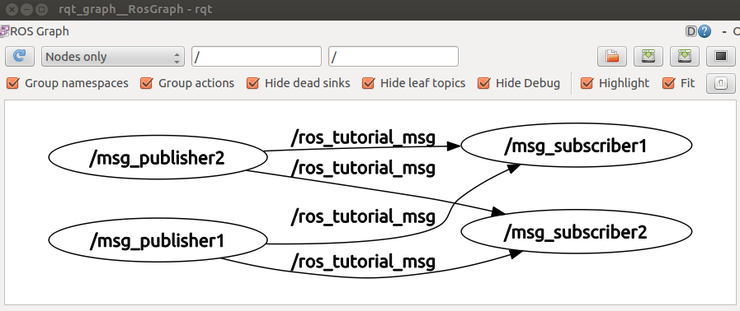
\includegraphics[width=12cm]{pictures/chapter6/pic_06_11.png}
  \caption{roslaunchを利用した複数のノードの実行}
\end{figure}

そこで、作成したunion.launchファイルを次のように変更する。

\begin{lstlisting}[language=ROS]
$ roscd irvs_ros_tutorials /launch
$ gedit union.launch
\end{lstlisting}

ファイル名: union.launch
\begin{lstlisting}[language=XML]
<launch>
<group ns = "ns1">
<node pkg = "irvs_ros_tutorials" type = "ros_tutorial_msg_publisher" name = "msg_publisher" />
<node pkg = "irvs_ros_tutorials" type = "ros_tutorial_msg_subscriber" name = "msg_subscriber" />
</group>

<group ns = "ns2">
<node pkg = "irvs_ros_tutorials" type = "ros_tutorial_msg_publisher" name = "msg_publisher" />
<node pkg = "irvs_ros_tutorials" type = "ros_tutorial_msg_subscriber" name = "msg_subscriber" />
</group>
</launch>
\end{lstlisting}

<group>タグは、指定されたノードをグループ化するタグである。オプションのnsには、名前空間(namespace)としてグループの名前を指定し、これによりグループに属するノードやメッセージの名前にnsタグの内容を付加する。もう一度、roslaunch コマンドでunion.launch を実行し、別のターミナルウインドウでrqt\_graphを起動して、ノード間の接続とメッセージの送受信の状態を確認してみよう。図6-12のような画面が表示され、最初に意図した通りの動作が確認できる。

\begin{lstlisting}[language=ROS]
$ roslaunch irvs_ros_tutorials union.launch --screen
\end{lstlisting}

\begin{lstlisting}[language=ROS]
$ rqt_graph
\end{lstlisting}

\begin{figure}[h]
  \centering
  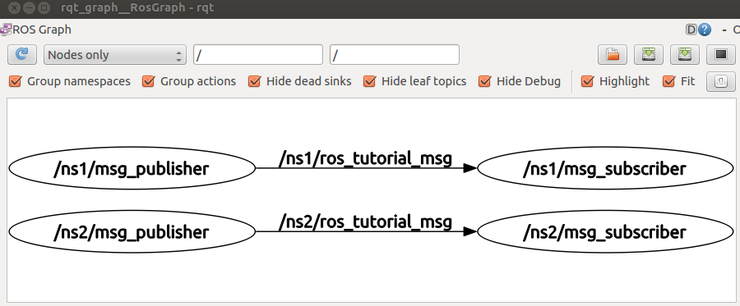
\includegraphics[width=12cm]{pictures/chapter6/pic_06_12.png}
  \caption{名前空間を用いたメッセージ通信}
\end{figure}

%-------------------------------------------------------------------------------
\subsection{launchファイルで使用されるタグ}

launchファイルは、XMLで記述することにより、ノードの動作を柔軟に制御できる。launchで使用されるタグを以下に挙げる。頻繁に使用されるタグについては既に説明しており、それ以外のタグの詳細もWiki\footnote{\url{http://wiki.ros.org/roslaunch/XML}}から確認できる。

\begin{itemize}
\item  <launch> : roslaunch構文の開始と終了を示す。
\item <node>: ノードを実行するためのタグである。パッケージ、ノード名、実行名を設定できる。
\item <machine>: ノードを実行しているPCの名前、address、ros-root、ros-package-pathなどを設定できる。
\item <include>: 他のパッケージや同じパッケージに属している他のlaunchファイルを読み込み、実行する。
\item <remap>: トピック名などのノードで使用しているROS変数の名前を変更する。
\item <env>: 環境変数を変更する。
\item <param>: パラメータの名、タイプ、値などを設定する。
\item <rosparam>: 4.4.5項で説明したrosparamコマンドのように、load、dump、deleteなどのパラメータ情報の確認と修正する際に使う。
\item <group>: 実行されているノードをグループ化するときに使用する。
\item <test>: ノードをテストするときに使用する。 <node>と似ているが、テストに使用できるオプションが追加されている。
\item <arg> : launchファイル内で変数を定義し、次の例のようにroslaunchコマンドの実行パラメータとして使うことができる。その際、パラメータは以下のように起動するlaunchファイル名後につける。例えばパラメータの名前(timing)と値(30)の間に「:=」をつけてパラメータの値を設定する。
\end{itemize}

\begin{lstlisting}[language=XML]
<launch>
  <arg name="update_ period" default="10" />
  <param name="timing" value="$(arg update_ period)"/>
</launch>
\end{lstlisting}

\begin{lstlisting}[language=ROS]
roslaunch my_file.launch timing:=30
\end{lstlisting}

%-------------------------------------------------------------------------------
